% Use the University of Michigan thesis class.
\documentclass[thesis]{./tex/thesis-umich}

% Title of the thesis
\title{Solving Nonlinear Equations of One Variable}

% Author name
\author{Derek J. Dalle}

% Department
\department{Aerospace Engineering}

% Year of completion
\year=2012

% Frontispiece
\frontispiece{FRONTISPIECE TEXT}

% Dedication
\dedication[4]{ %
This dissertation is in honor of Adlai Stevenson and William Jennings Bryan,
who were both twice the Democratic nominee for President of the United States
without winning either time.  As an interesting side note, Adlai Stevenson's
grandfather, Adlai E. Stevenson I, was William Jennings Bryan's
running mate in the 1900 election.}

% Acknowledgments
\acknowledgments[4]{ %
It is imperative that I thank all of the authors of the dissertation
template from the Department of Atmospheric, Oceanic and Space Sciences, 
which is available online at
\href{http://aoss.engin.umich.edu/pages/current/dissertation-template}{ %
http://aoss.engin.umich.edu/}.  To my knowledge, the authors include
Jin Ji, Roque D. Oliveira, and Jason Gilbert.  I also must thank Sara
Spangelo for suggesting that this template be ready by the end of April 2011.
}
\acknowledgmentswidth{0.8}

% Preface
\preface{ %
The text of this document is of course mainly meant to show how
the template works.  The topic is thus a basic problem which has
been solved in a large number of ways.  This sample topic, which
is solving equations of one variable using iterative techniques,
allows us to use sample equations and figures so that we can see
how they will look in this template.  In addition to the standard
methods, the text also demonstrates a new algorithm that has
slightly improved performance.}

% Committee
\committee{ %
Professor James F. Driscoll, Chair \\
Professor Peter J. Olver, University of Minnesota}

% Commands to hide or show lists of figures, tables, etc.
\hidelistoftables
\showlistofappendices

% Definition of any abbreviations used.
\abbreviations{
 \acro{CFD}{Computational Fluid Dynamics}
 \acro{MSRSF}{Monotonic, Single-Root Scalar Function}
}

%% DOCUMENT AREA
\begin{document}


\chapter{Introduction}   \label{chap:intro}
The first part.  For example in \ac{CFD}.

\begin{figure}
 \begin{center}
  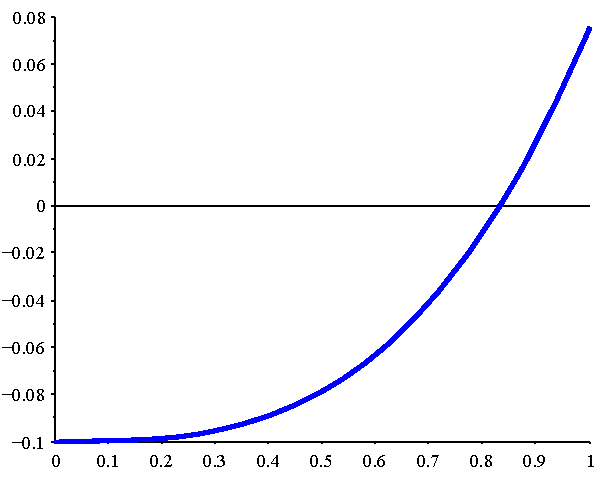
\includegraphics[scale=1]{./pics/f1_plain.pdf}
 \end{center}
 \caption{ \label{fig:fn:1}
  An example of a search function}
\end{figure}

\newpage

And this should at least continue onto a second page.  There are many texts that have a section on the subject, for instance \cite{chapra:2002:numerics}.

\chapter{Setting}
The second chapter has the good stuff.

\section{Convergence Criteria}
Actually, it might have the worst stuff.  But it is slightly easier to write than the material in Chapter \ref{chap:intro}.

\begin{figure}
 \begin{center}
  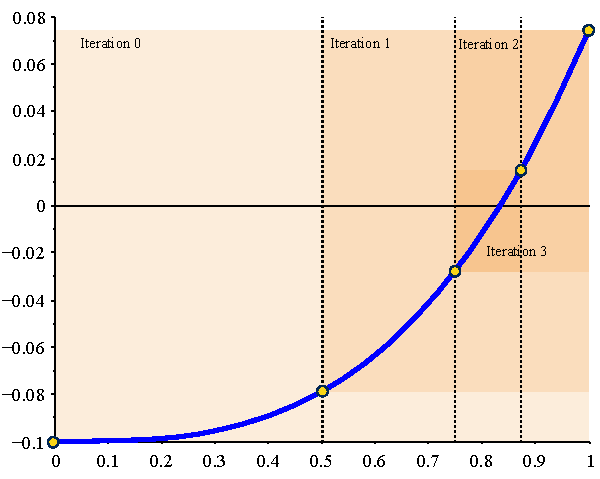
\includegraphics[scale=1]{./pics/f1_tol.pdf}
 \end{center}
 \caption{ \label{fig:fn:tol}
  Illustration of $x$- and $y$-tolerances for bisection iterations}
\end{figure}

\newpage

It takes very little text to fill a page in this format, but there is even less text on most of these sample pages.

\section{Why we are doing it}
It is usually a good idea to give reasons for your research.  If you do not, the people who payed you to waist all that time will feel really bad about it, and then they will not provide the same opportunity to future students.

\newpage

I need this page to see what even-numbered pages look like.

\appendix
\chapter{Methods}
Here is how to implement the methods.

\section{Bisection}
The easiest method.

\section{False Position}
The next one.

% Using AIAA bibliography style since I'm in aero.
\bibliographystyle{aiaa}
% Give this command the relative path to the .bib file.
\bibliography{./tex/thesis-bib}

\end{document}